\documentclass[final]{beamer}
\usetheme{RJH}
\usepackage[orientation=portrait,size=a1,scale=1.3,debug]{beamerposter}
\usepackage[absolute,overlay]{textpos}
\usepackage{amsmath}
\usepackage{mathtools}
\usepackage{commath}
\usepackage[font=scriptsize,labelfont=bf]{caption}
\usepackage{multicol}
\setlength{\TPHorizModule}{1cm}
\setlength{\TPVertModule}{1cm}
\setbeamertemplate{caption}[numbered]
\setbeamertemplate{itemize items}[ball]
\setbeamertemplate{bibliography item}{\insertbiblabel}

\title{Dynamical systems modeling of the child–mother dyad:\\ \vspace{0.15em}
Causality between child-directed language complexity \\ 
\vspace{0.15em}
and language development \vspace{0.15em}}
%\author{{\large \bf Jeremy Irvin \qquad Daniel Spokoyny} \\
%\vspace{0.2em}
%  College of Creative Studies\\ \vspace{0.2em}
%  {\large \bf Ferm\'{\i}n Moscoso del Prado Mart\'{\i}n } \\ \vspace{0.3em}
%  Department of Linguistics}
\footer{}
\author[shortname]{Jeremy Irvin 
%\inst{1} 
\and Daniel Spokoyny 
%\inst{1} 
\and Ferm\'{\i}n Moscoso del Prado Mart\'{\i}n 
%\inst{2}
}
%\institute[shortinst]{\inst{1} College of Creative Studies \and %
%                      \inst{2} Department of Linguistics}
\date{}

\begin{document}
\begin{frame}{} 

\begin{textblock}{10}(1,4.5)

\includegraphics[width=6.5cm]{ccs.png}
\end{textblock}

\begin{textblock}{10}(50,4.8)

\includegraphics[width=8.5cm]{ling.jpg}
\end{textblock}

\begin{textblock}{22}(1,9)
\begin{block}{Abstract}
We model the \emph{causal} links between child language (CL) and child-directed language (CDL). We take pairs of sequences of linguistic measurements from a longitudinal study \cite{MacWhinney14, Theakston01}. Each child-mother pair of sequences is considered as an instance of the trajectory of a high-dimensional dynamical system. We then use Multispatial Convergent Cross Mapping \cite{Clark15} to ascertain the directions of causality between the pairs of sequences, that is, whether the complexity of CL drives that of CDL, the complexity of CDL drives that of CL, both, or neither.
\end{block}

\begin{block}{Background}
\begin{itemize}
\item \text{ }Child-directed language (``motherese'')
\item \text{ }Fine-tuning \cite{Snow89, Sokolov93} (Weak or Strong)
\end{itemize}
\vspace{1cm}
\hrule
\vspace{1cm}
\begin{multicols}{2}
\text{ }
\begin{figure}
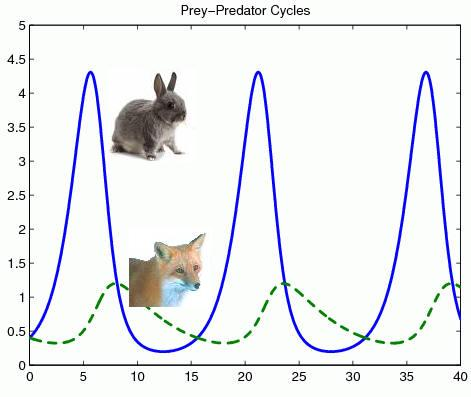
\includegraphics[width=10cm]{pred_prey.jpg}
\caption{Example of a simple dynamical system with two variables.}
\label{fig:predprey}
\end{figure}
\columnbreak
\small
\begin{itemize}
\item \text{ }Dynamical systems models describe the co-evolution of multiple variables over time (Fig.~\ref{fig:predprey})
\item \text{ }Typically described by a system of coupled differential equations
\item \text{ }Linguistic and behavioral interaction between parent-child dyads can be jointly considered as part of a single dynamical system \cite{VanGeert91}
\end{itemize}
\normalsize
\end{multicols}
\end{block}

\begin{block}{Causality Detection in Dynamical Systems}
\begin{figure}
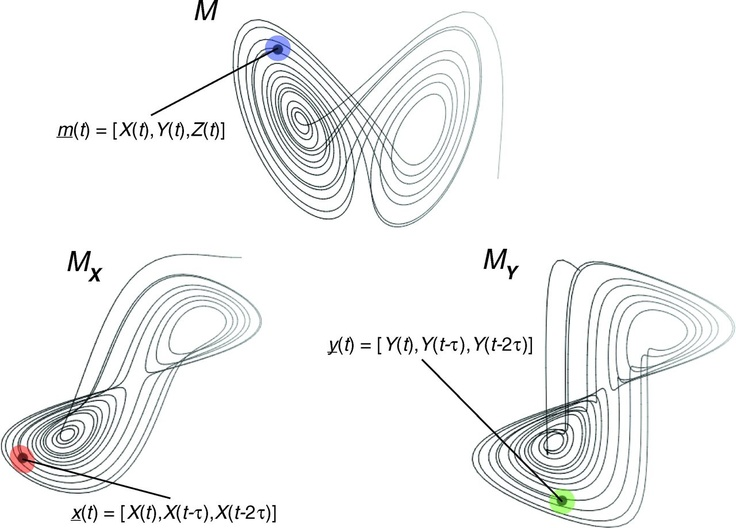
\includegraphics[width=14cm]{lorenz2.jpg}
\hspace{0.5em}
\raisebox{0.3\height}{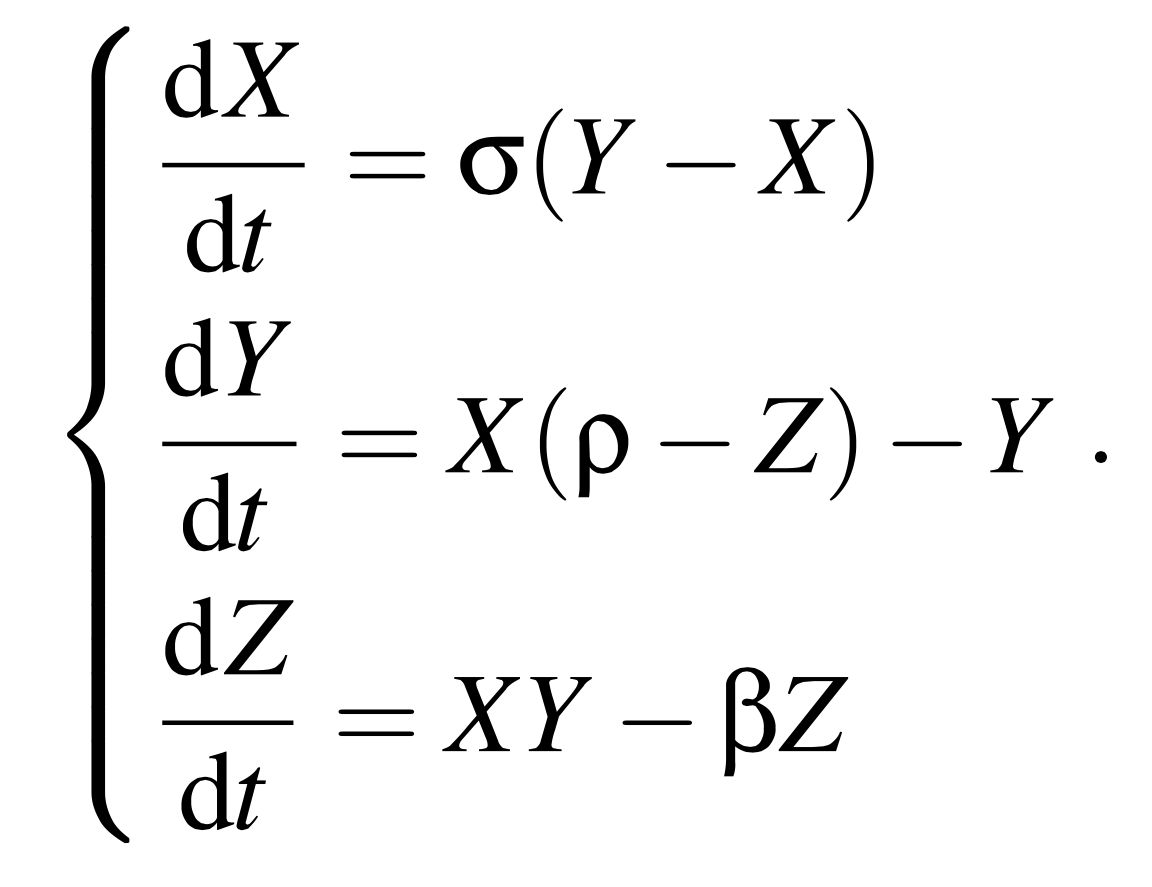
\includegraphics[width=7cm]{lorenz.png}}
\hspace{0.5em}
%\hspace{2em}
%\footnotesize
%\begin{equation*}
%\begin{dcases}
%\dod{X}{t} = \sigma ( Y - X ) \\[10pt]
%\dod{Y}{t} = X (\rho - Z) - Y \\[10pt]
%\dod{Z}{t} = X Y - \beta Z 
%\end{dcases}.
%\label{eq:lorenz}
%\end{equation*}
%\normalsize
\caption{Reconstructed manifold for Lorenz’s system ($M$; top), as well as the shadow manifolds reconstructed considering only $X$ ($M_X$ ; bottom-left) and $Y$ ($M_Y$ ; bottom-right) \cite{Sugihara12}.}
\label{fig:lorenz}
\end{figure}
\vspace{-1.5cm}
\begin{multicols}{2}
\footnotesize
\begin{itemize}
\item \text{ }\emph{Convergent Cross Mapping}
\item \text{ }Non-separable systems
\item \text{ }Robust to noise
\item \text{ }\textbf{Can discern direct causality from shared driving variables}
\end{itemize}
\columnbreak
\begin{itemize}
\item \text{ }Not all relevant variables available
\item \text{ }Instead of $(X[t], Y[t], Z[t])$, $(X[t+\tau], ..., X[t+\tau(E-1)])$ \cite{Takens81} (Fig.~\ref{fig:lorenz})
\item \text{ }Nearby points on $Y$ identify nearby points on $X$ \cite{Sugihara12}
\end{itemize}
\normalsize
\end{multicols}
\end{block}
\end{textblock}

\begin{textblock}{34}(24.5,9)
\begin{block}{Methods and Materials}
\begin{itemize}
\item \text{ }Manchester Corpus \cite{MacWhinney14} from CHILDES database \cite{Theakston01}
\begin{itemize}
\item \text{ }Longitudinal study of 12 children (6 girls and 6 boys) between 2 and 3 years old
\item \text{ }For each child and mother, the total number of words, the lexical diversity \cite{Moscoso14}, and the mean length of the utterances (MLU) were recorded (Fig.~\ref{fig:evolution})
\end{itemize}
\end{itemize}
\begin{figure}
\begin{tabular}{ccc}
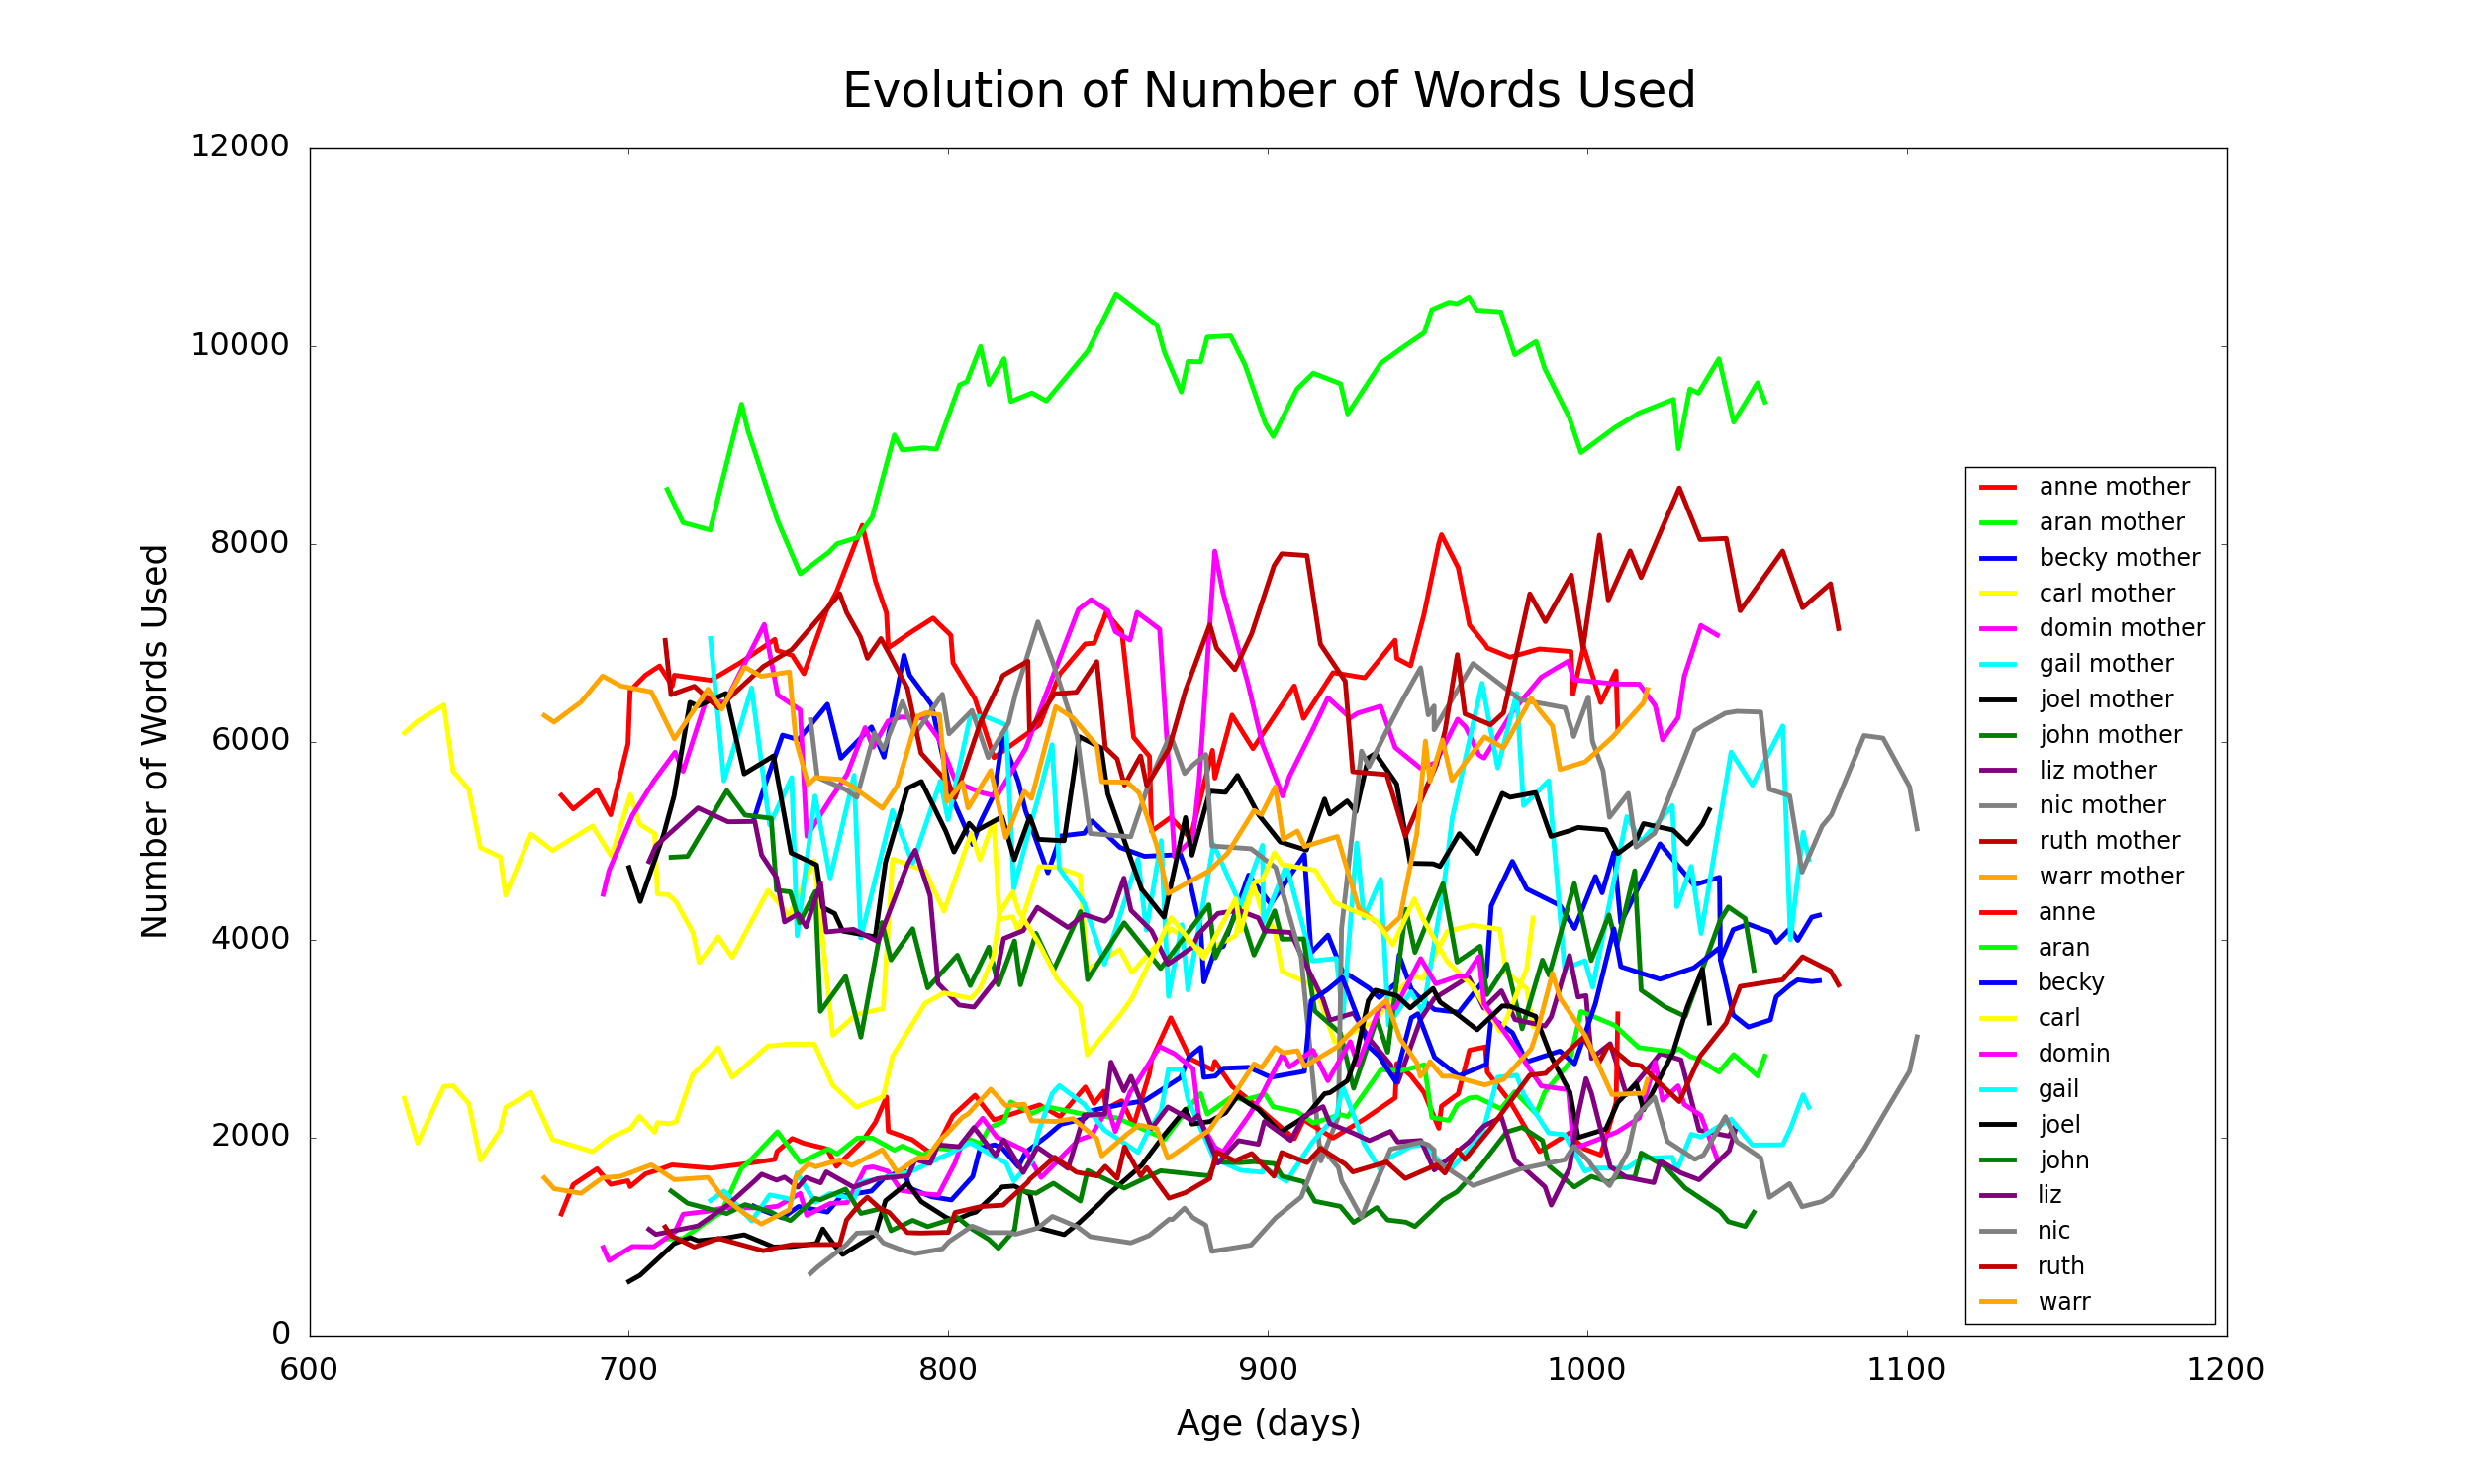
\includegraphics[width=.325\textwidth]{nwords_evolution.png} &
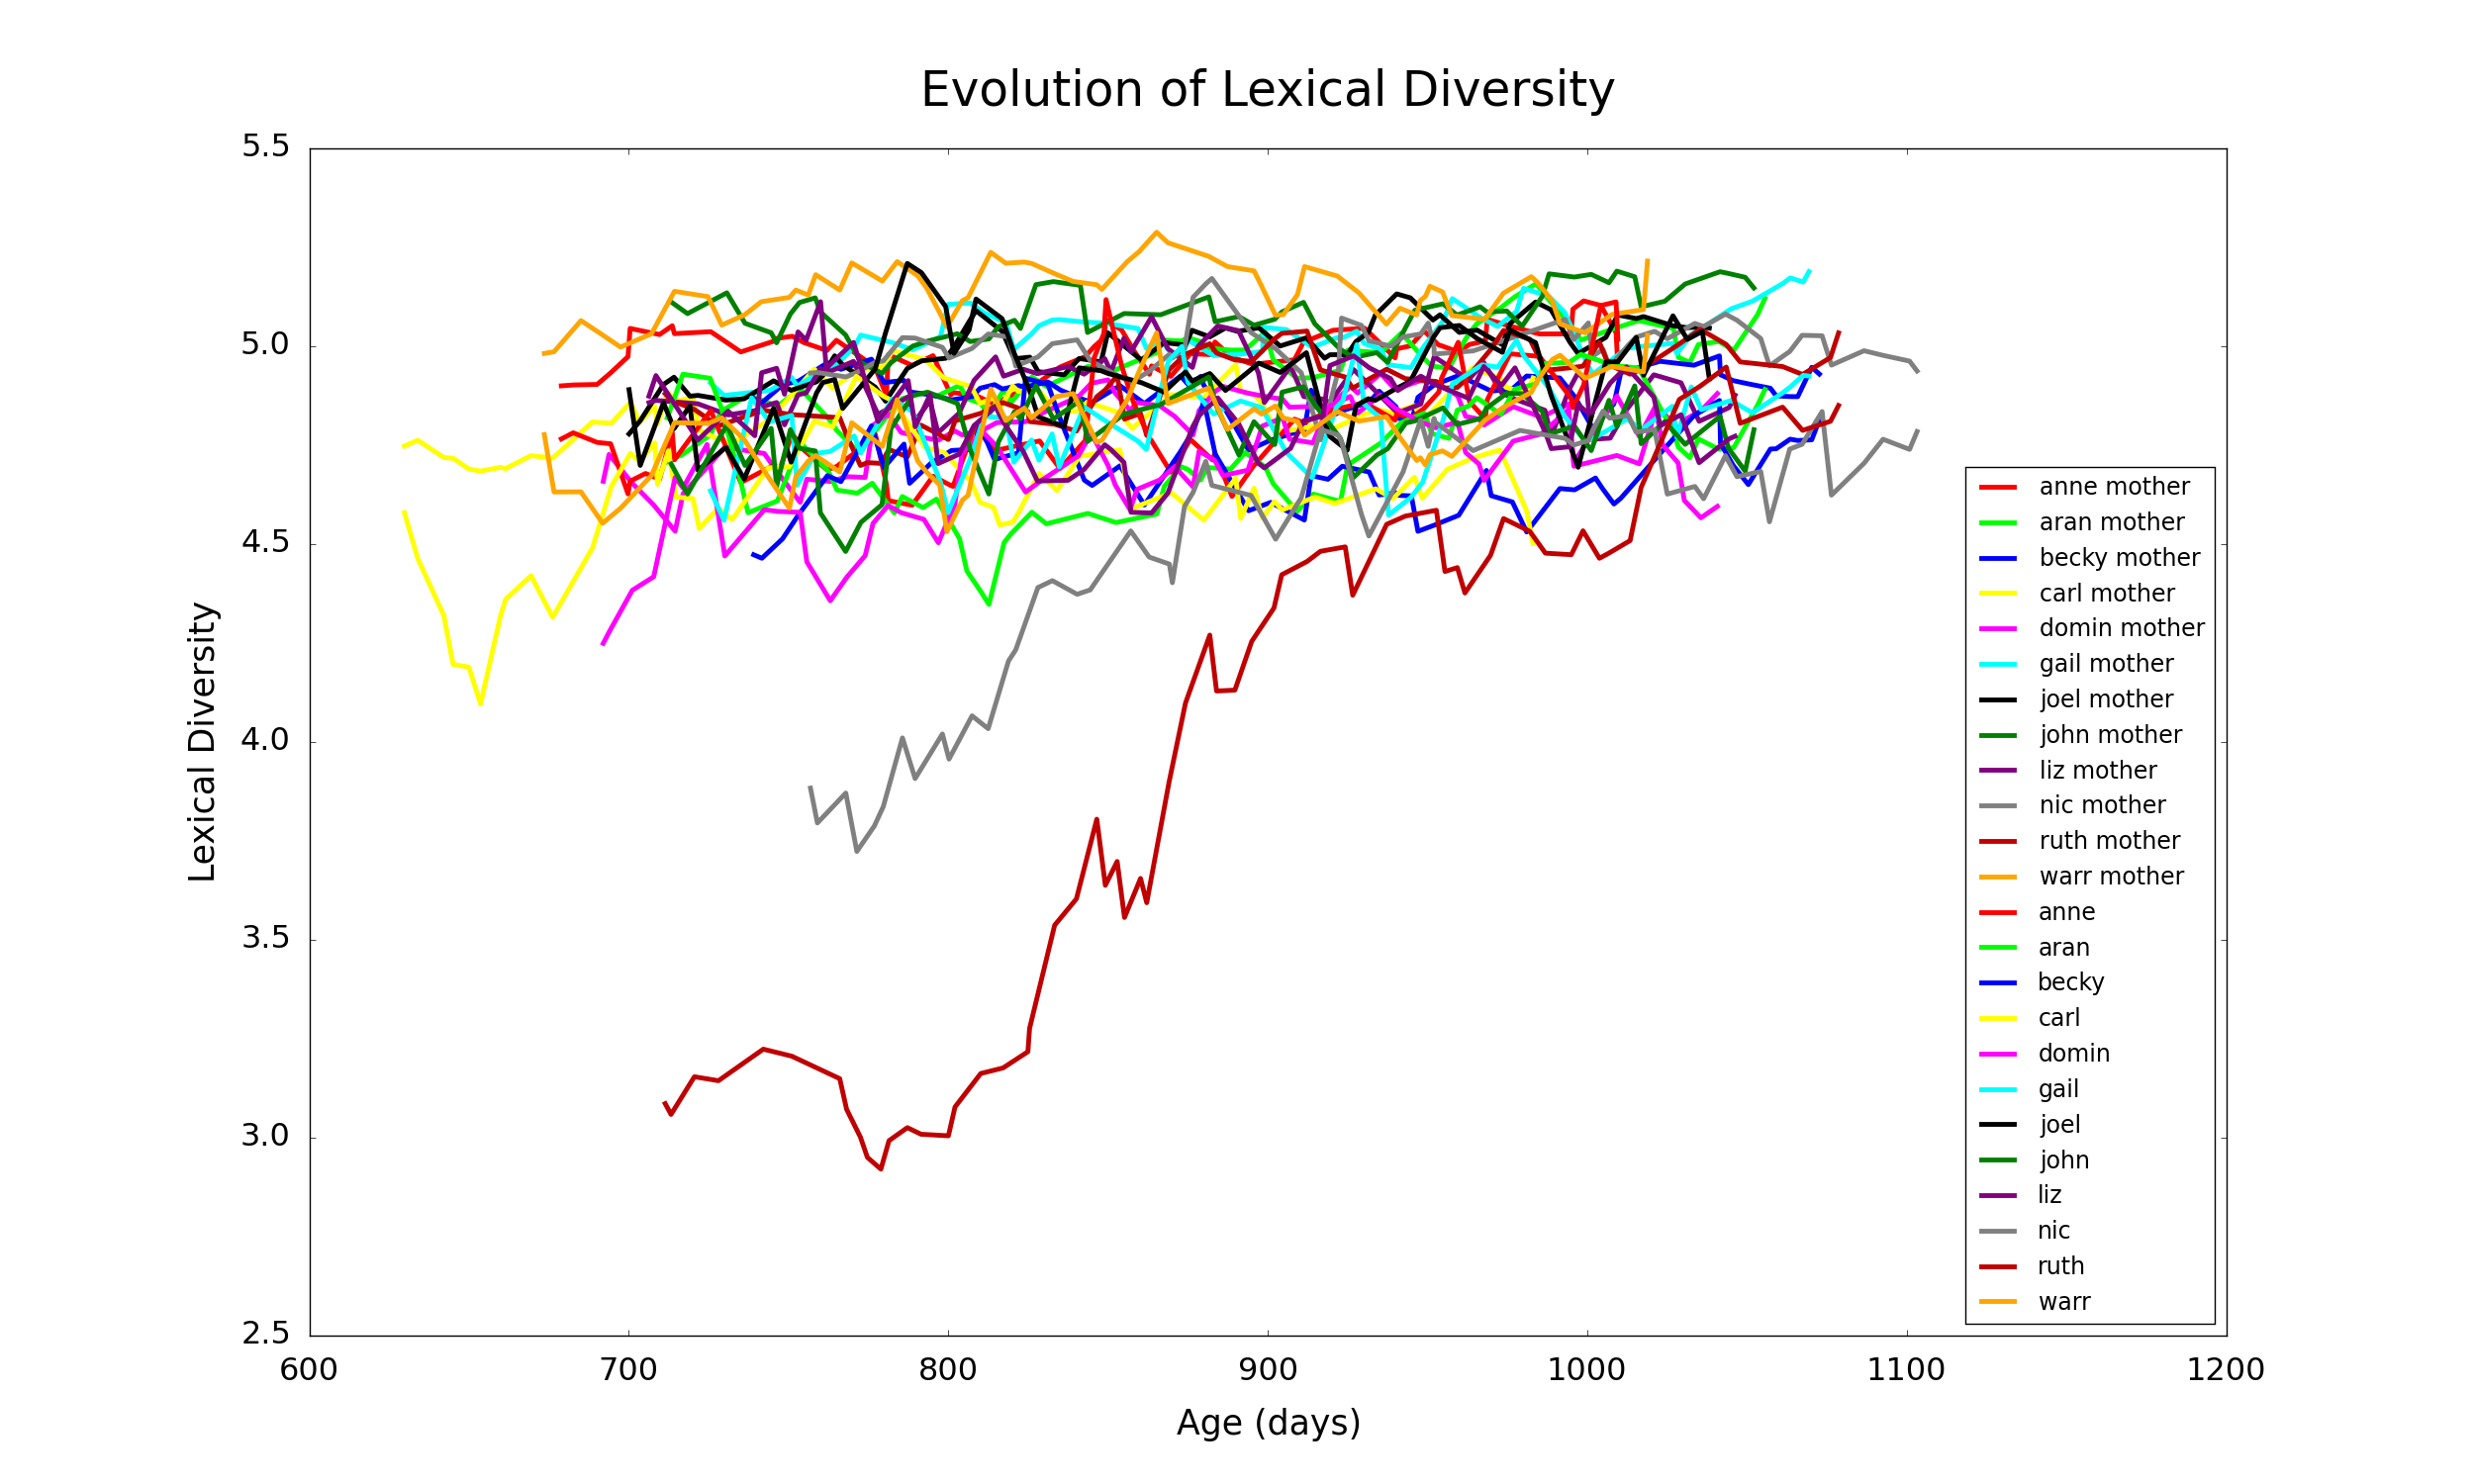
\includegraphics[width=.325\textwidth]{lexical_evolution.png} &
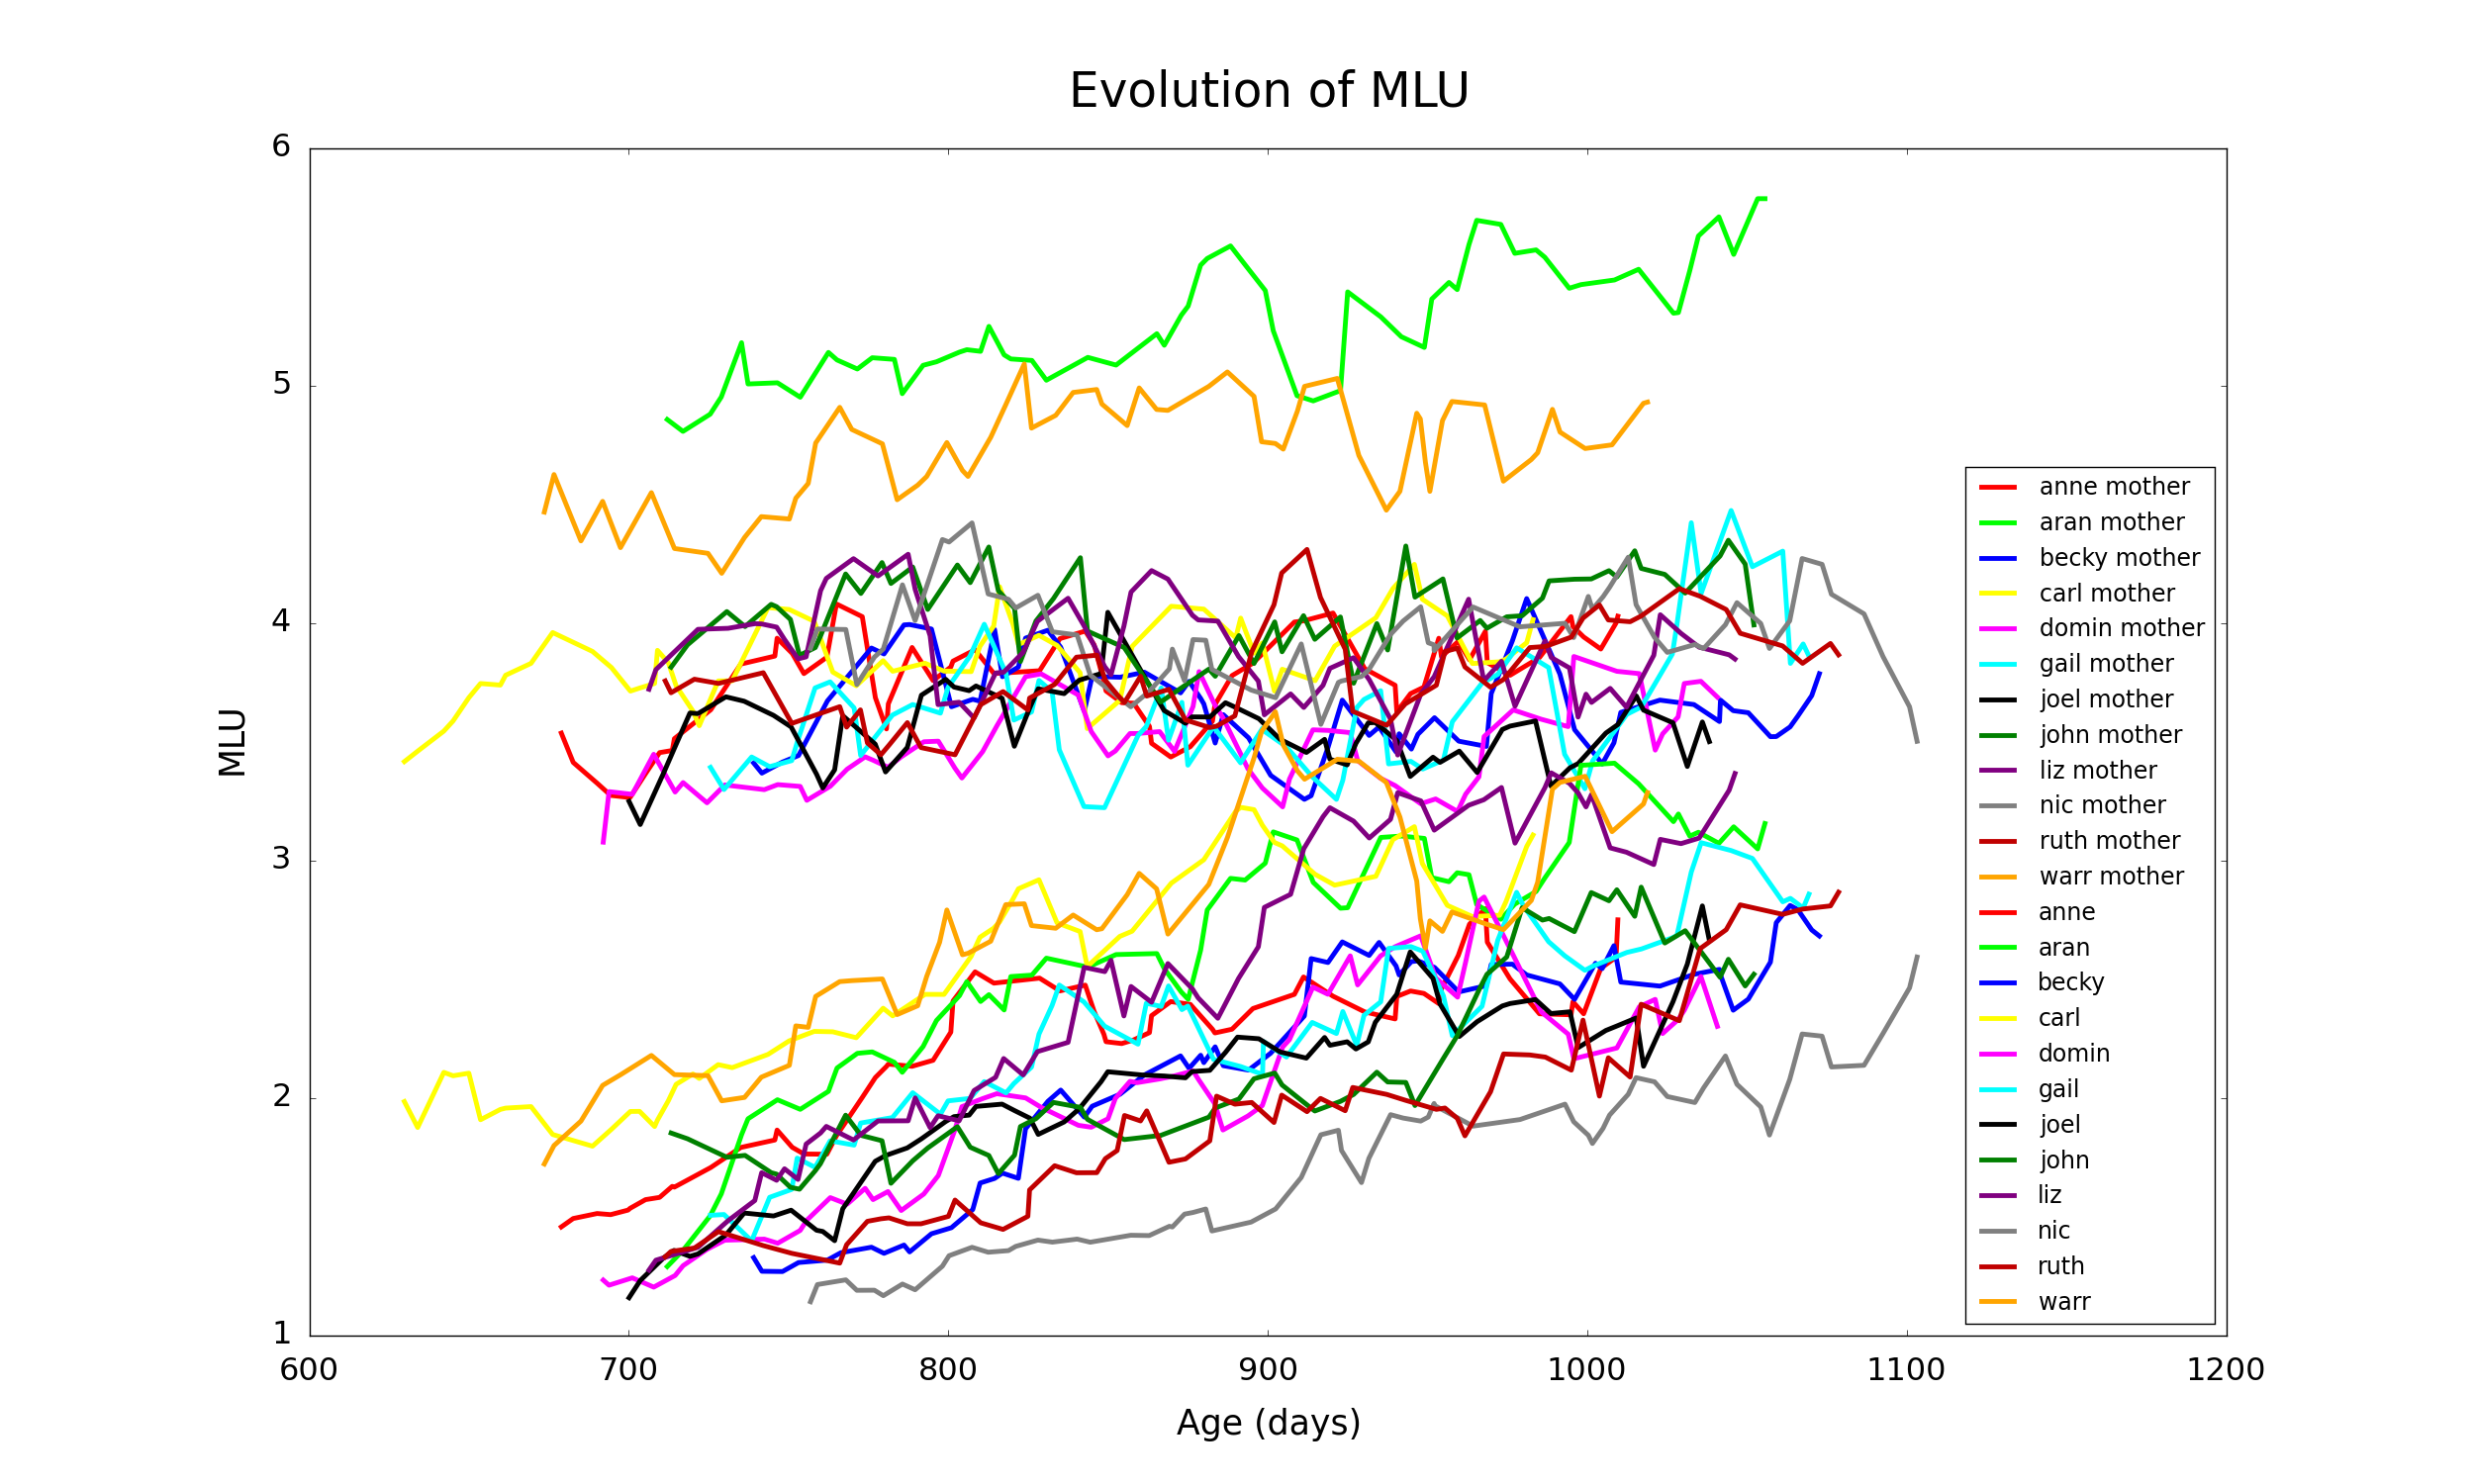
\includegraphics[width=.325\textwidth]{syntactic_evolution.png}
\end{tabular}
\caption{Evolution of the measures under consideration as a function of the children's ages, for the children (bottom curves) and their mothers (top curves).}
\label{fig:evolution}
\end{figure}
\begin{itemize}
\item \text{ }Embedding reconstruction of time series
\begin{itemize}
\item \text{ }Parameters were not found to differ significantly across children or mothers, so used a single estimate $(\tau, E)$ for all children and one for all mothers
\end{itemize}
\end{itemize}
\begin{itemize}
\item \text{ }Multispatial CCM Causality Detection (mCCM) \cite{Clark15}
\begin{itemize}
\item \text{ }Directional causality between children's and mothers' measures tested using mCCM  (1000 bootstrapping iterations to assess $p$-values)
\item \text{ }$p$-values adjusted for multiple corrections using false discovery rate \cite{Benjamini01}
\end{itemize}
\end{itemize}
\end{block}

\begin{block}{Results}
\begin{figure}
\begin{tabular}{ccc}
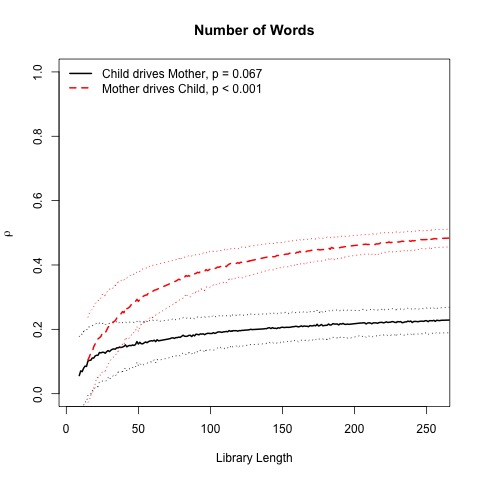
\includegraphics[width=.32\textwidth]{N_Words_Cause.jpg} &
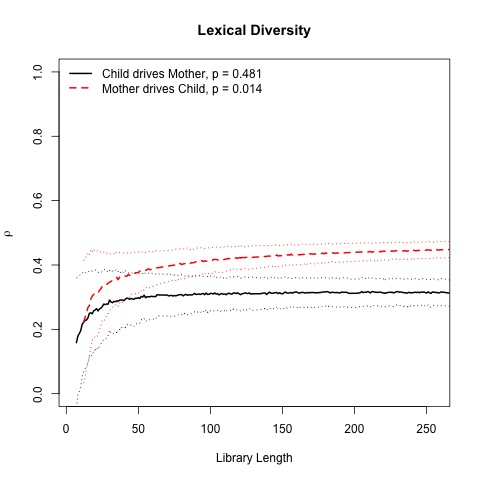
\includegraphics[width=.32\textwidth]{Lexical_Cause.jpg} &
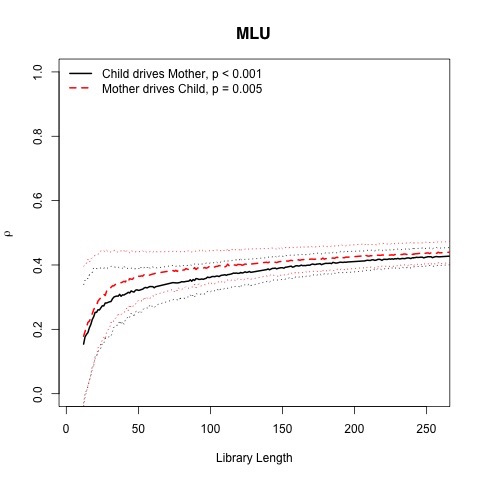
\includegraphics[width=.32\textwidth]{Syntactic_Cause.jpg} \\
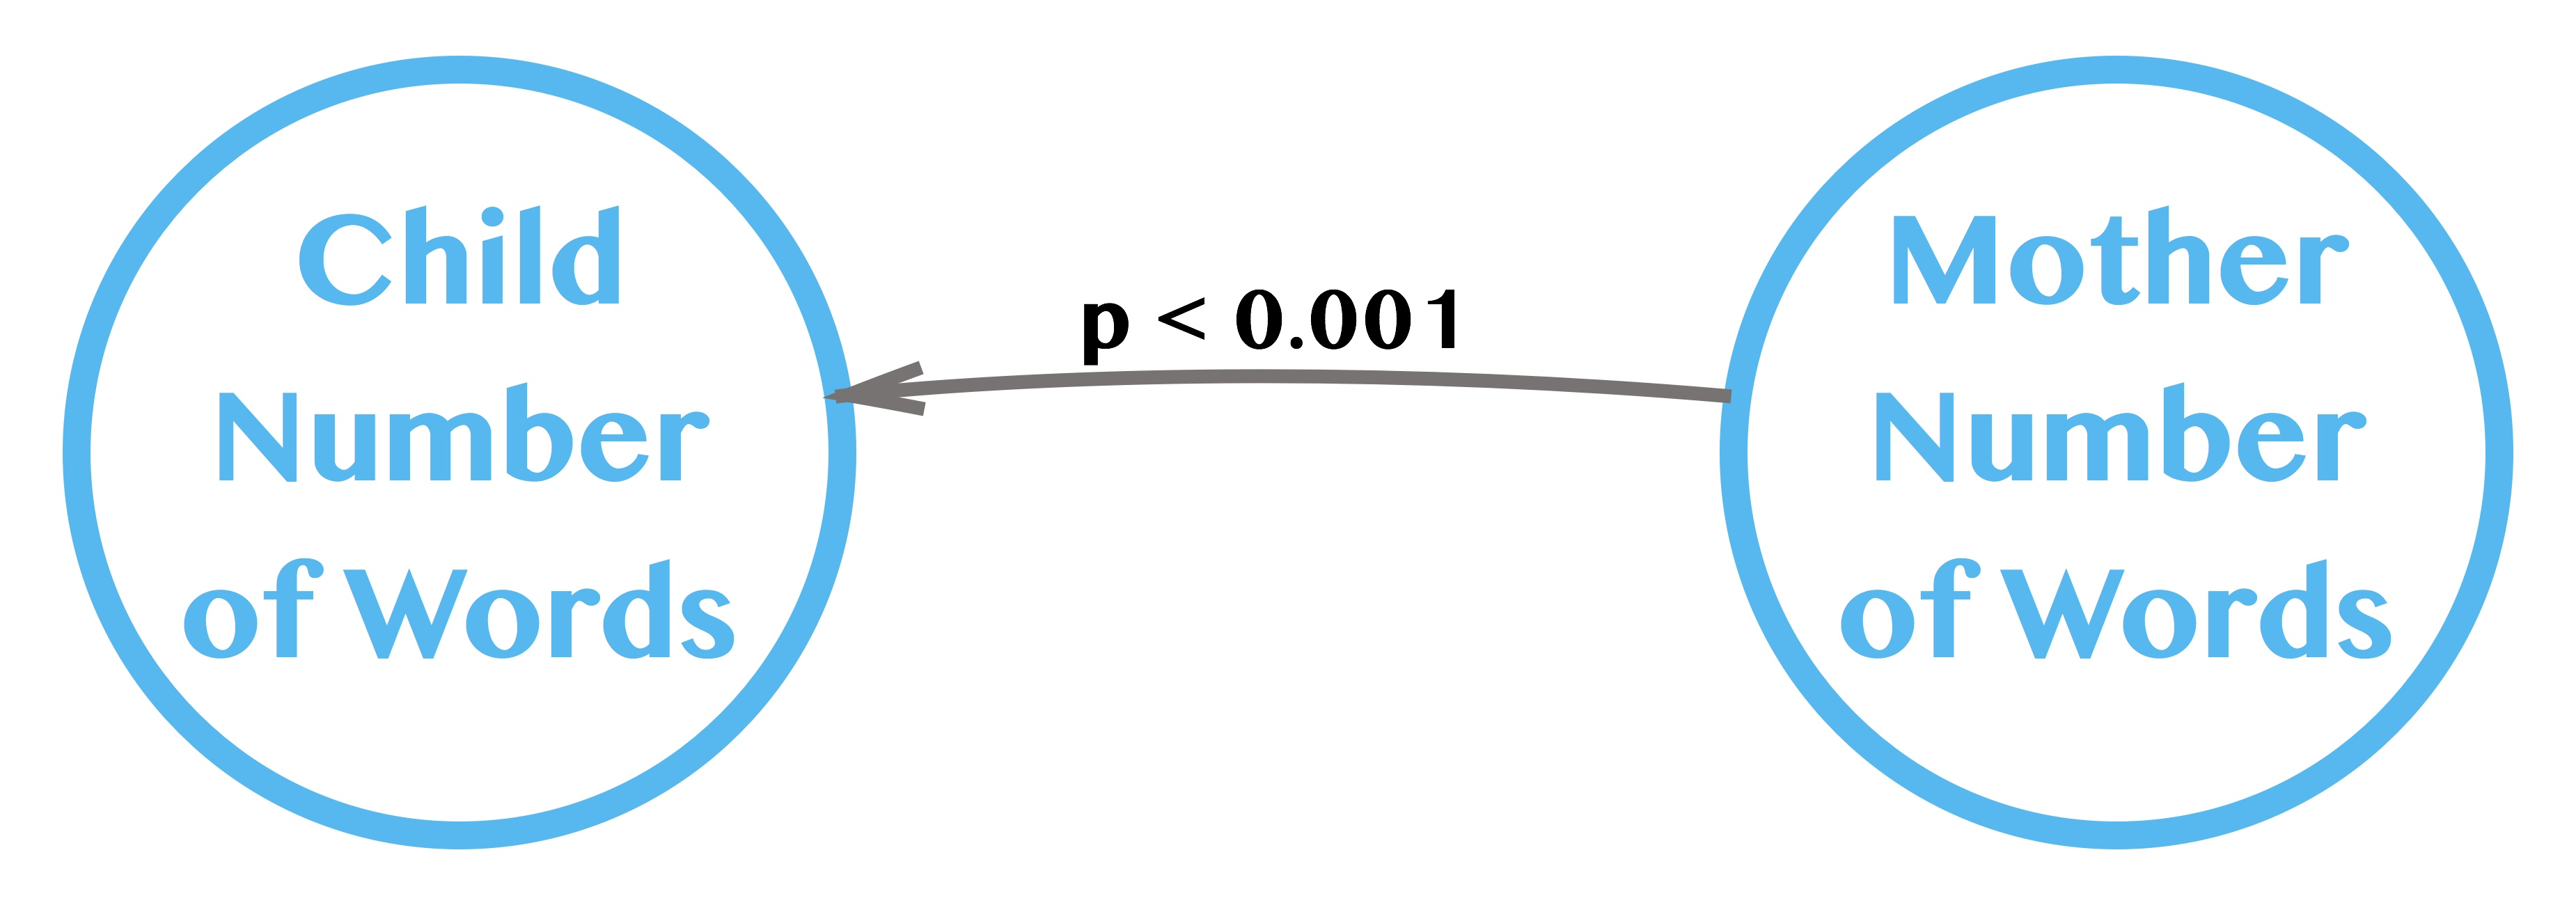
\includegraphics[width=.32\textwidth]{loq_results.jpg} & 
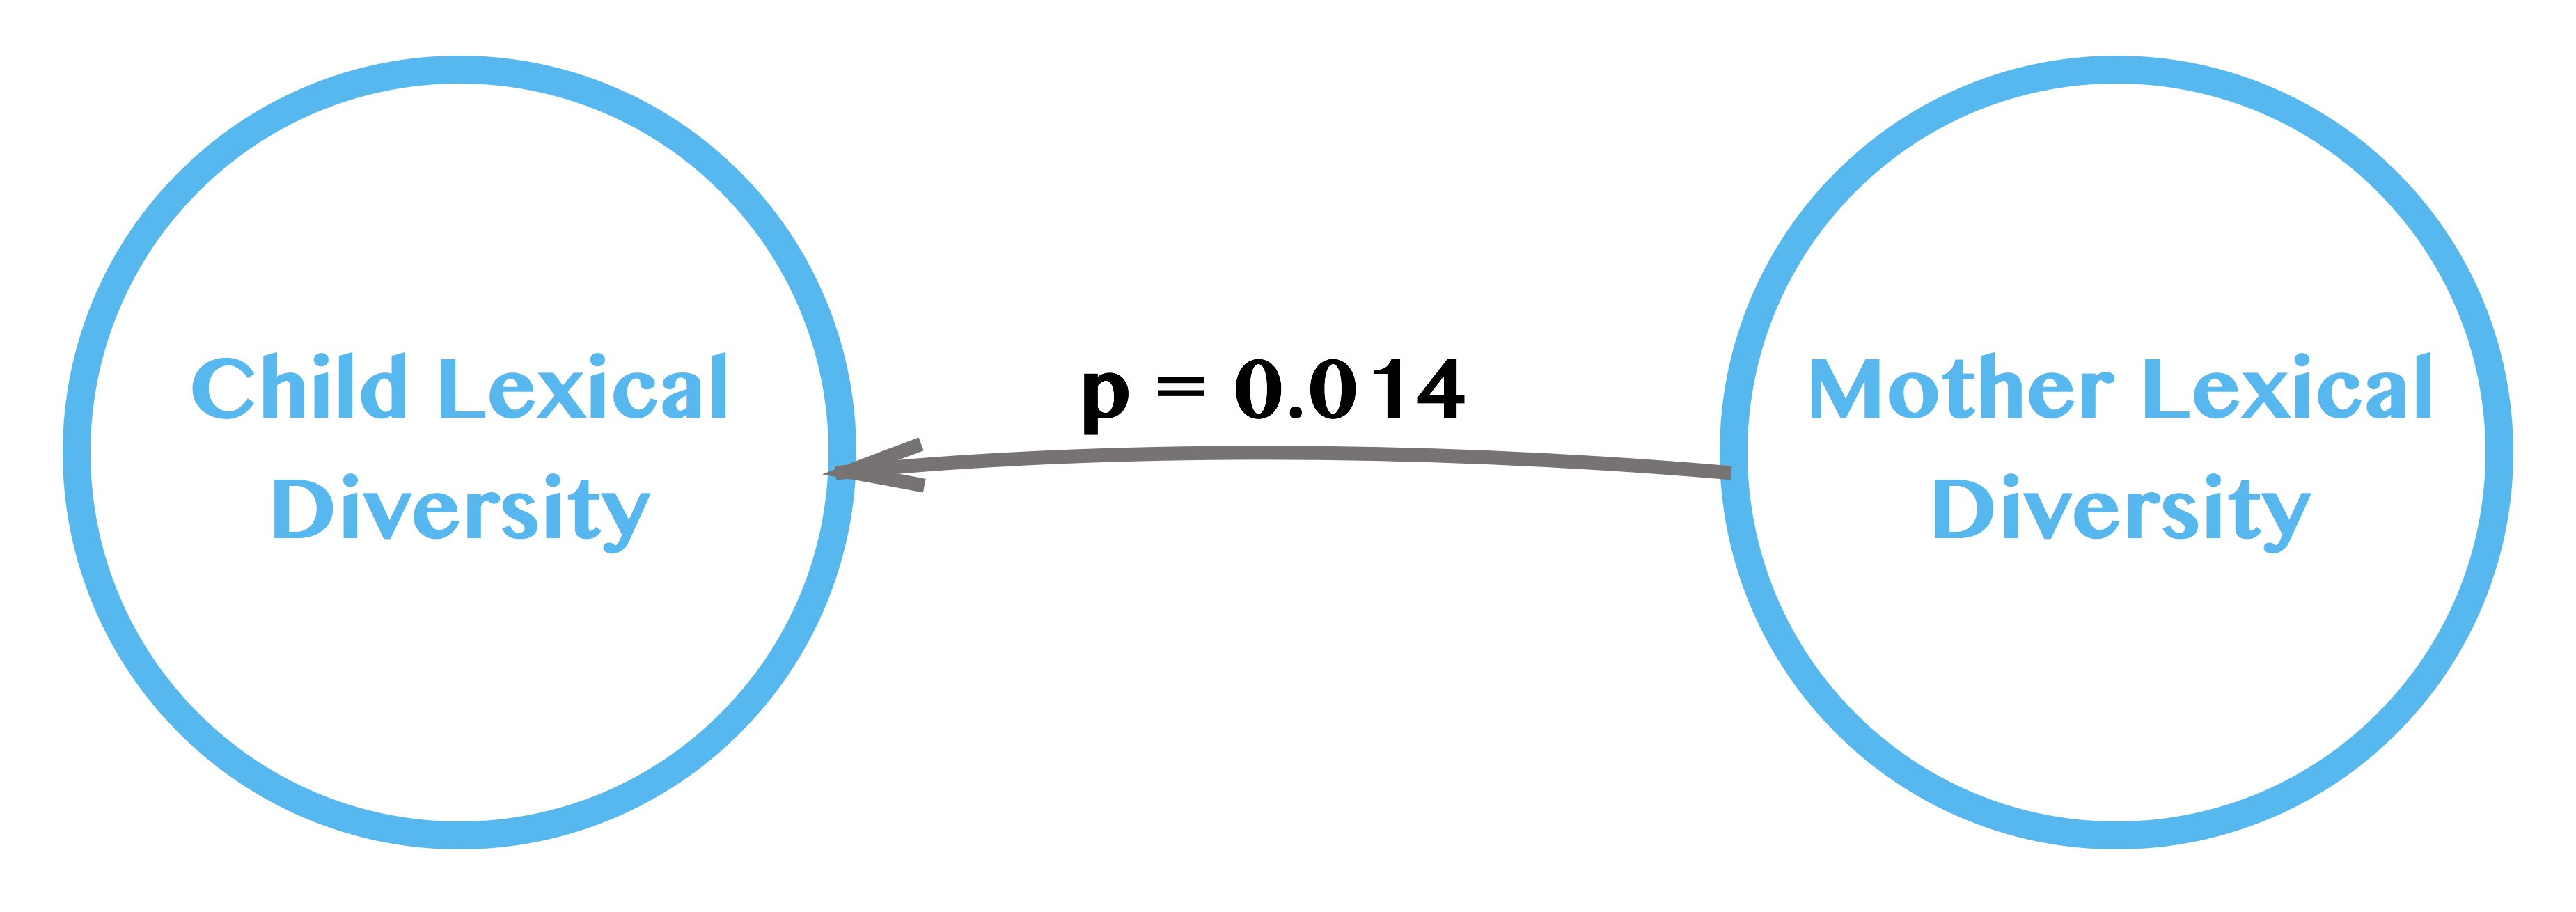
\includegraphics[width=.32\textwidth]{lex_results.jpg} &
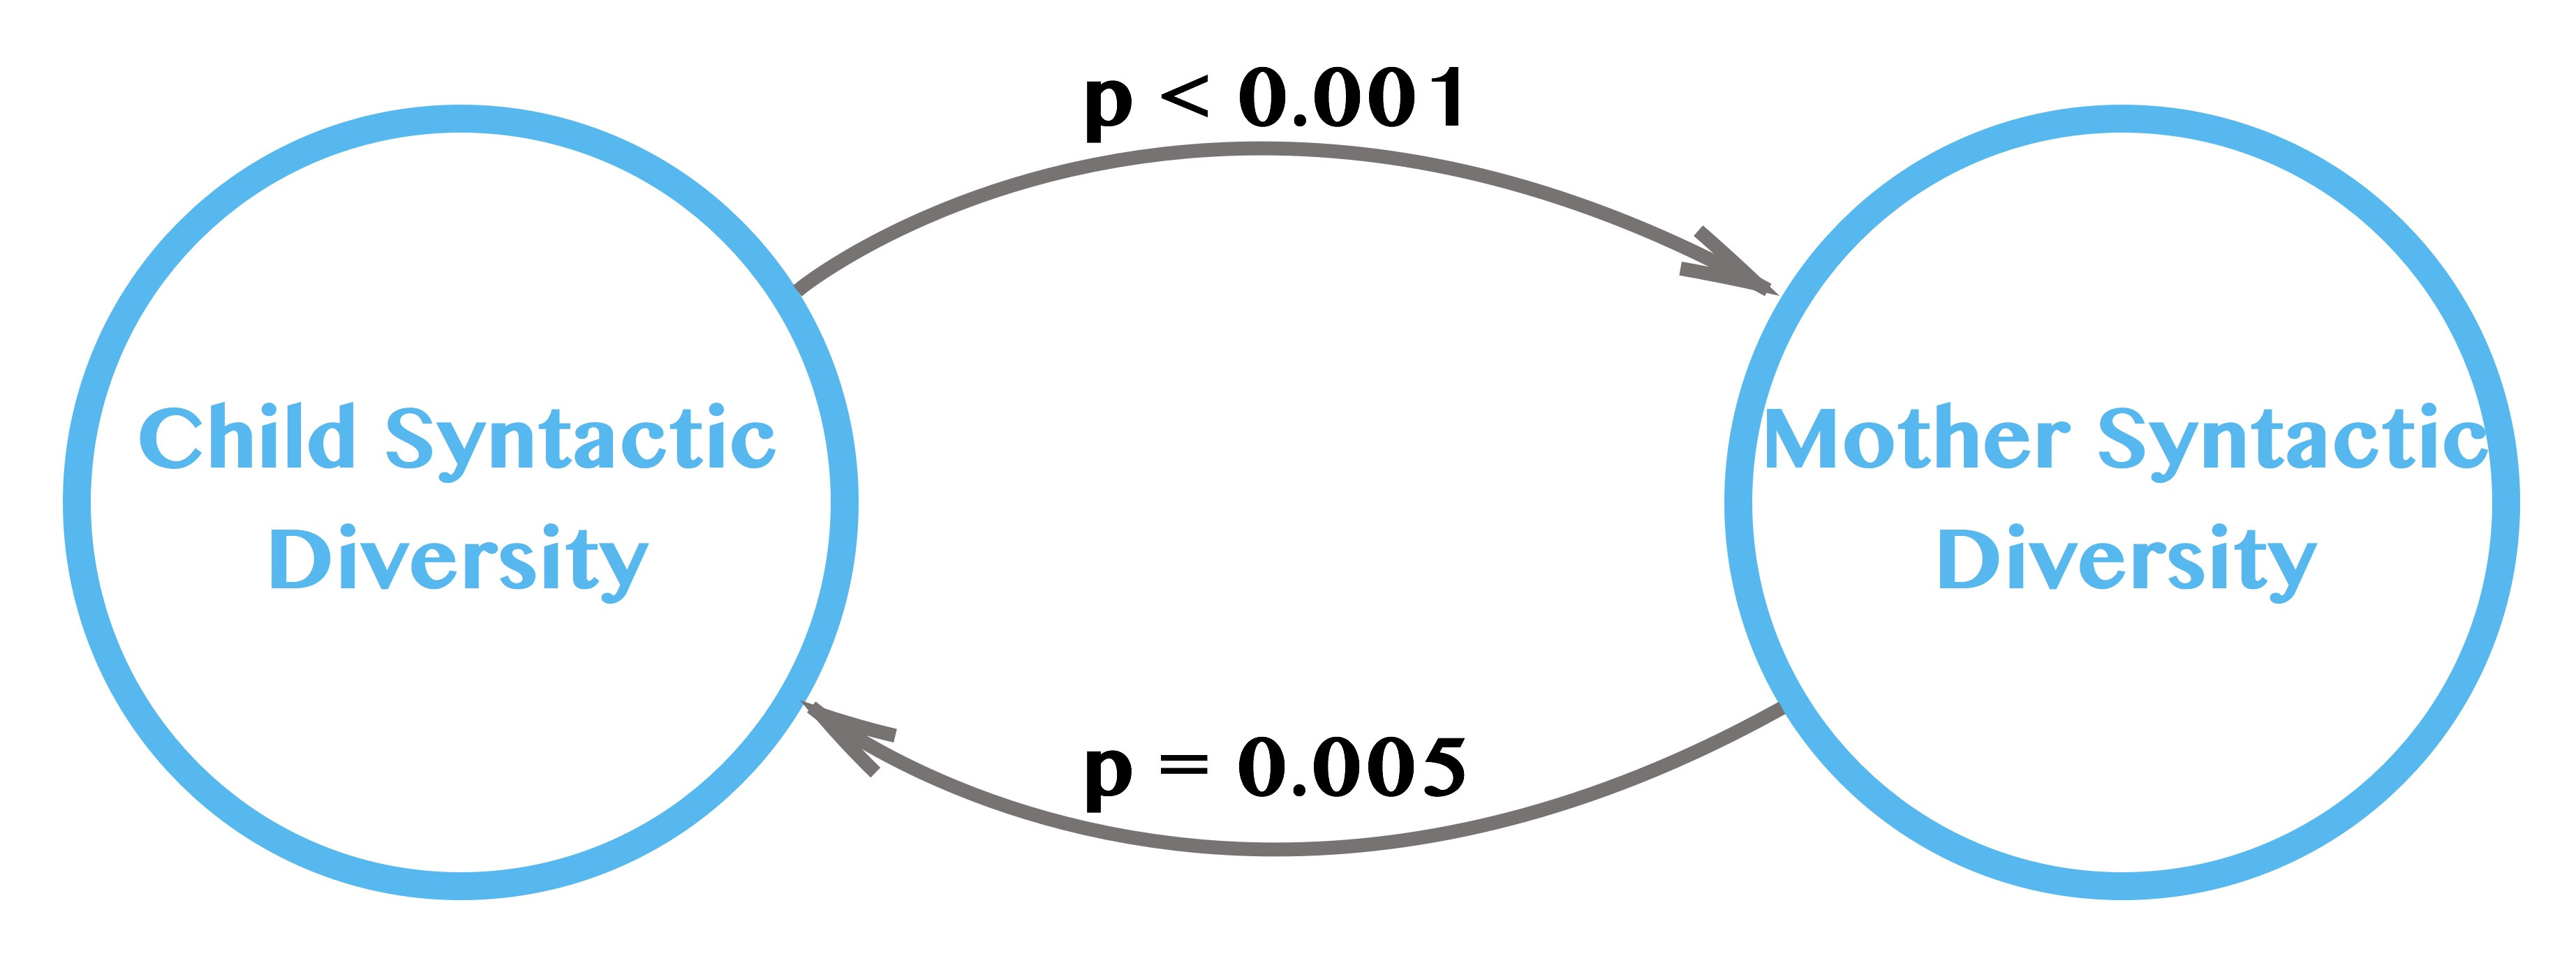
\includegraphics[width=.32\textwidth]{mlu_results.jpg}
\end{tabular}
\caption{For each of the measures considered, we plot the evolution of Pearson’s correlation coefficient ($\rho$) between the predicted and predicting shadow manifolds. The dashed lines denotes the standard deviation of the estimates. A value of $\rho$ significantly increasing with library length is mCCM’s indication of causality between two variables.}
\label{fig:results}
\end{figure}

\begin{itemize}
\item \text{ }\textbf{Evidence found for both weak and strong fine-tuning}
\end{itemize}

\end{block}

\begin{block}{References}\vspace{-1.3cm}
\begin{multicols}{2}
{\tiny
\bibliography{mybib}}
\end{multicols}
\bibliographystyle{unsrt}
\end{block}

\end{textblock}

\end{frame}
\end{document}
